
\documentclass[preprint,12pt]{elsarticle}

\usepackage[spanish]{babel}
\usepackage{amssymb}
\usepackage{graphicx}
\usepackage{lineno}
\usepackage[utf8]{inputenc}
\usepackage{url}
\usepackage{natbib} 
\usepackage{amsmath} 
\usepackage{amssymb} 

\begin{document}
	
	\begin{frontmatter} 

		\title{\huge Gestores de BD NoSQL}
		
		\author{Estrella Palacios, Katherine Lizbeth      (2016056193))}
		\author{Andia Zeballos,Alonso André           	(2016054945))}
		\author{Porlles Carrillo, Diego Armando	         	(2015050948))}  
		\author{Mamani Mamani, Pedro Luis                 (2010038808))} 
		\address{Escuela Profesional de Ingeniería de Sistemas}
		\address{Universidad Privada de Tacna}
		\address{Tacna, Perú}
		
%% ABSTRACT --------------------------------------------------------------------------------------------------------------------

		\begin{abstract}
		
NoSQL databases have experienced a significant increase in their application in recent times. The great flexibility they offer and the possibilities they offer from the point of view of optimization in their designs according to the problem to be solved make them an attractive variant to consider for developers of information management applications. In this article, we take a look at the evolution of the types of databases until they reach the relational ones, which are analyzed in order to show the aspects associated with them that led to the emergence of the NoSQL. v

		\end{abstract}

%% ----------------------------------------------------------------------------------------------------------------------------------

	\end{frontmatter}

%% RESUMEN ---------------------------------------------------------------------------------------------------------------------

\section{Resumen}

Las bases de datos NoSQL han experimentado un importante incremento en su aplicación en los últimos tiempos. La gran flexibilidad que ofrecen y las posibilidades que brindan desde el punto de vista de la optimización en sus diseños de acuerdo al problema a resolver las convierten en una atractiva variante a tener en cuenta para los desarrolladores de aplicaciones de gestión de información. En el presente artículo se hace un recorrido por la evolución de los tipos de bases de datos hasta llegar a las relacionales, las cuales se analizan con el objetivo de mostrar los aspectos asociados a estas que propiciaron el surgimiento de las NoSQL.

%% ----------------------------------------------------------------------------------------------------------------------------------


%% INTRODUCION ----------------------------------------------------------------------------------------------------------------

\section{Introducción} 





%% ----------------------------------------------------------------------------------------------------------------------------------


%% MARCO TEÓRICO ------------------------------------------------------------------------------------------------------------

\section{Marco Teórico}

%% PRIMERA SUBSECCION 

\subsection {\textbf{Definición}}

Una base de datos no relacional (NoSQL) es aquella base de datos que:

\begin{itemize}
	\item No requiere de estructuras de datos fijas como tablas
	\item No garantiza completamente las características ACID
	\item Escala muy bien horizontalmente.
\end{itemize}

Se utilizan en entornos distribuidos que han de estar siempre disponibles y operativos y que gestionan un importante volumen de datos.

%% https://revistadigital.inesem.es/informatica-y-tics/los-gestores-de-bases-de-datos-mas-usados/

\subsubsection{\textbf{A1}}

EDITAR\\

%%Ejemplo de cita
\cite{Gartner} 


\begin{itemize}
	\item x
	\item y
	\item z
\end{itemize}

\subsubsection{\textbf{A2}}

EDITAR\\

\subsubsection{\textbf{A3}}

EDITAR\\


%% SEGUNDA SUBSECCION

\subsection{\textbf{B}}

\subsubsection{\textbf{B1}}

EDITAR\\

%% Ejemplo de inclusión de imagen
\begin{figure}[htb]
	\begin{center}
		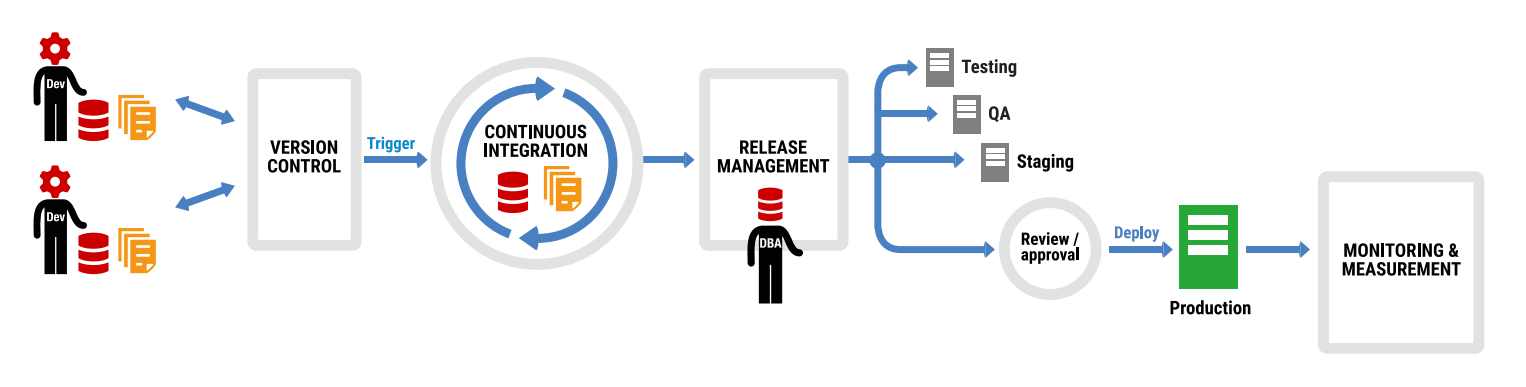
\includegraphics[width=14cm]{./IMAGENES/basededatos_1} 
		\caption{Incluyendo la base de datos en DevOps}
	\end{center}
\end{figure}

\subsubsection{\textbf{B2}}

EDITAR\\

%% TERCERA SUBSECCION
\subsection{\textbf{C}}

\subsubsection{\textbf{C1}}

EDITAR\\

\begin{itemize}

\item x
\item y
\item z

\end{itemize}
\subsubsection{\textbf{C2}}

EDITAR\\


%% ----------------------------------------------------------------------------------------------------------------------------------
 


%% ANÁLISIS ( APLICACIÓN ) ---------------------------------------------------------------------------------------------------

\section{Análisis}

\subsection{\textbf{Análisis 1}}
EDITAR\\

\subsection{\textbf{Análisis 2}}
EDITAR\\

\subsection{\textbf{Análisis 3}}
EDITAR\\

\subsection{\textbf{Análisis 4}}
EDITAR\\

%% ----------------------------------------------------------------------------------------------------------------------------------


%% CONCLUSIONES ---------------------------------------------------------------------------------------------------------------

\section{Conclusiones}

\begin{itemize}

\item Conclusion 1 : \\

\item Conclusion 2 : \\ 

\item Conclusion 3 : \\ 

\item Conclusion 4 : \\ 
\end{itemize}

%% ----------------------------------------------------------------------------------------------------------------------------------

%%  REFERENCIAS BIBLIOGRÁFICAS ------------------------------------------------------------------------------------------
	
	\newpage
	
	\bibliographystyle{apalike} 	%ESTILO
	\bibliography{BIBLIOGRAFIA}	 
	
	
\end{document}
